\documentclass[12pt, hidelinks]{article}
\usepackage[brazil]{babel}
\usepackage[utf8]{inputenc}
\usepackage{amsmath}
\usepackage{natbib}
\usepackage{listings}
\usepackage{color}

\definecolor{codegreen}{rgb}{0,0.6,0}
\definecolor{codegray}{rgb}{0.5,0.5,0.5}
\definecolor{codepurple}{rgb}{0.58,0,0.82}
\definecolor{backcolour}{rgb}{0.95,0.95,0.92}

\lstdefinestyle{mystyle}{
  backgroundcolor=\color{backcolour},
  commentstyle=\color{codegreen},
  keywordstyle=\color{red},
  numberstyle=\tiny\color{codegray},
  stringstyle=\color{codepurple},
  basicstyle=\footnotesize,
  breakatwhitespace=false,
  breaklines=true,
  captionpos=b,
  keepspaces=true,
  numbers=left,
  numbersep=5pt,
  showspaces=false,
  showstringspaces=false,
  showtabs=false,
  tabsize=2,
  extendedchars=true,
  literate={á}{{\'a}}1 {ã}{{\~a}}1 {õ}{{\~o}}1 {é}{{\'e}}1 {ç}{{\c{c}}}1,
}

\lstset{style=mystyle}
\usepackage{url}
\usepackage{amsmath}
\usepackage{float}
\usepackage{graphicx}
\graphicspath{{images/}}
\usepackage{parskip}
\usepackage{fancyhdr}
\usepackage{vmargin}
\usepackage{hyperref}
\setmarginsrb{3 cm}{2.5 cm}{3 cm}{2.5 cm}{1 cm}{1.5 cm}{1 cm}{1.5 cm}


\title{Sistemas de Equações Lineares}								% Title
\author{Wilton Rodrigues}								% Author
\date{\today}											% Date

\makeatletter
\let\thetitle\@title
\let\theauthor\@author
\let\thedate\@date
\makeatother

\pagestyle{fancy}
\fancyhf{}
\lhead{\centering{\thetitle}}
\cfoot{\thepage}

\begin{document}

%%%%%%%%%%%%%%%%%%%%%%%%%%%%%%%%%%%%%%%%%%%%%%%%%%%%%%%%%%%%%%%%%%%%%%%%%%%%%%%%%%%%%%%%%

\begin{titlepage}
  \centering
  \begin{figure}[H]
    \centering
    
\includegraphics[width=0.7\textwidth]{figuras/logo.png}\\[2.0 cm]
  \end{figure}
  \textsc{\LARGE Universidade de Brasília}\\[2.5 cm]	% University Name
  \textsc{\Large Relatório de atividade do módulo 2}\\[0.5 cm]				% Activity name
  \textsc{\large Métodos Numéricos para Engenharia}\\[1.5 cm]				% Course Name
  \rule{\linewidth}{0.2 mm} \\[0.4 cm]
  {\huge \bfseries \thetitle}\\
  \rule{\linewidth}{0.2 mm} \\[2.5 cm]

  \begin{minipage}{0.4\textwidth}
    \begin{flushleft} \large
      \emph{Aluno:}\\
      \theauthor
    \end{flushleft}
  \end{minipage}
  \begin{minipage}{0.4\textwidth}
    \begin{flushright} \large
      \emph{Matrícula:} \\
      13/0049212									% Your Student Number
    \end{flushright}
  \end{minipage}\\
  \vspace*{0.5in}
  {\large \thedate}\\[0.5 cm]

  \vfill

\end{titlepage}

%%%%%%%%%%%%%%%%%%%%%%%%%%%%%%%%%%%%%%%%%%%%%%%%%%%%%%%%%%%%%%%%%%%%%%%%%%%%%%%%%%%%%%%%%

\section{Introdução}

O objetivo deste relatório é exercitar os conceitos aprendidos em aula, com relação ao tópico: \thetitle.
Que tem como objetivo prover métodos matemáticos capazes de solucionar esses sistemas que aparecem frequentemente
em matemática aplicada, economia e na modelagem de fenônemos na engenharia.
O problema a ser solucionado é o circuito mostrado abaixo, que é conhecido como Ponte de Wheatstone, e é frequentemente usado em medidas eletrônicas.

\begin{figure}[!h]
  \centering
  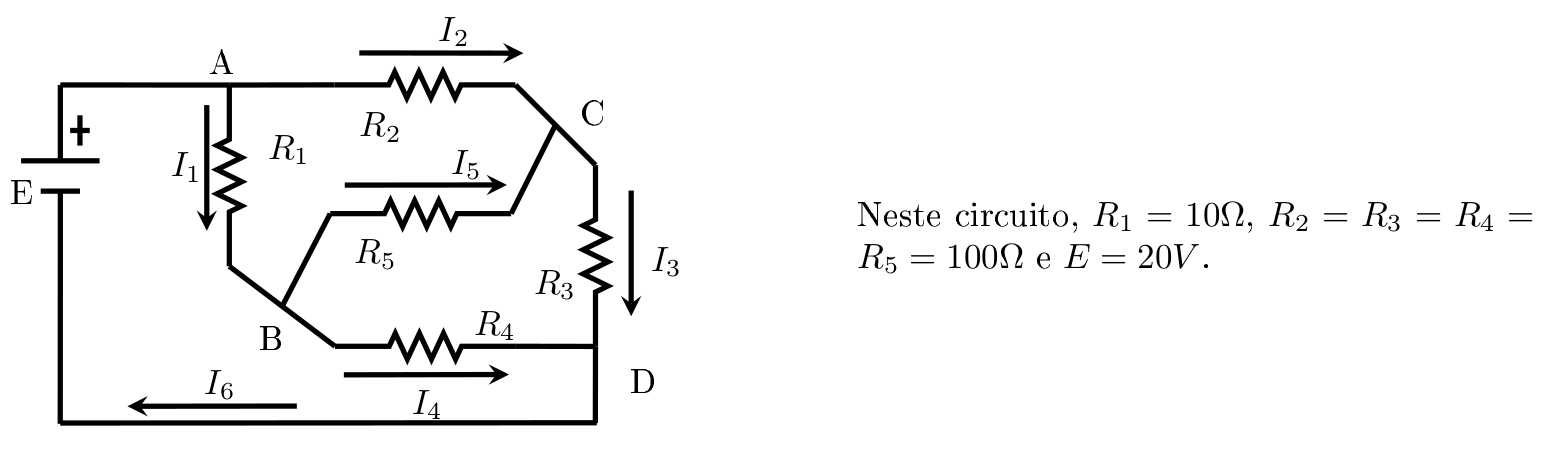
\includegraphics[width=15cm]{figuras/problema.png}\\
  \caption{Ponte de Wheatstone}\label{fig:ponte}
\end{figure}

De acordo com os dados do problema, as equações que governam o problema são obtidas a partir da Lei de Kirchoff.
Sendo assim, para as seguintes malhas temos as seguintes equações:
\begin{eqnarray}\label{eq:sistema}
  Para~ABD: & I_1R_1+I_4R_4-E=0 \nonumber\\
  Para~ABCA: & I_1R_1+I_5R_5-I_2R_2=0 \nonumber\\
  Para~BCDB: & I_5R_5+I_3R_3-I_4R_4=0 \nonumber\\
  Para~o~A: & I_6=I_1+I_2 \nonumber\\
  Para~o~B: & I_1=I_5+I_4 \nonumber\\
  Para~o~C: & I_3=I_2+I_5
\end{eqnarray}

O objetivo do trabalho é solucionar o sistema de equações lineares acima para determinar as correntes
$I1, I2,...,I6$ através do método de eliminação de Gauss-Jordan, com uma precisão de 10 casas decimais.

\section{Metodologia}

A primeira coisa a se fazer é passar o sistema de equação~\eqref{eq:sistema} para o formato matricial, sendo assim obtemos a seguinte relação:
\begin{eqnarray}\label{eq:matrizes}
  R * I = E
\end{eqnarray}
Onde $R$ é a matriz dos resistores, $I$ é o vetor das Correntes e $E$ o vetor das tensões.
A partir da relação expressa na equação~\eqref{eq:matrizes} obtemos a seguinte matriz:
\begin{eqnarray}\label{eq:matrizes2}
\left[\begin{array}{rrrrrr}
R_1 & R_2 & R_3 & R_4 & R_5 & R_6\\
R_1 & R_2 & R_3 & R_4 & R_5 & R_6\\
R_1 & R_2 & R_3 & R_4 & R_5 & R_6\\
R_1 & R_2 & R_3 & R_4 & R_5 & R_6\\
R_1 & R_2 & R_3 & R_4 & R_5 & R_6\\
R_1 & R_2 & R_3 & R_4 & R_5 & R_6
\end{array}\right] *
\left[\begin{array}{r}
I_1\\I_2\\I_3\\I_4\\I_5\\I_6
\end{array}\right] =
\left[\begin{array}{r}
E_1\\E_2\\E_3\\E_4\\E_5\\E_6
\end{array}\right]
\end{eqnarray}
Baseando-se nos valores iniciais informados na figura~\eqref{fig:ponte} para as resistências e a tensão ao fazermos as devidas
substituições obtemos a seguinte expressão:
\begin{eqnarray}\label{eq:matrizes3}
\left[\begin{array}{rrrrrr}
10 & 0 & 0 & 100 & 0 & 0\\
10 & -100 & 0 & 0 & 100 & 0\\
0 & 0 & 100 & -100 & 100 & 0\\
-1 & -1 & 0 & 0 & 0 & 1\\
1 & 0 & 0 & -1 & -1 & 0\\
0 & -1 & 1 & 0 & -1 & 0
\end{array}\right] *
\left[\begin{array}{r}
I_1\\I_2\\I_3\\I_4\\I_5\\I_6
\end{array}\right] =
\left[\begin{array}{r}
20\\0\\0\\0\\0\\0
\end{array}\right]
\end{eqnarray}
Pela qual é possível expressar qualquer uma das equações informadas inicialmente no sistema~\eqref{eq:sistema}. Ao pegarmos a
matriz $R$ e o vetor $E$ teremos a matriz aumentada $MA$:
\begin{eqnarray}\label{eq:matrizes3}
\left[\begin{array}{rrrrrrrr}
10 & 0 & 0 & 100 & 0 & 0 & \vdots & 20\\
10 & -100 & 0 & 0 & 100 & 0 & \vdots & 0\\
0 & 0 & 100 & -100 & 100 & 0 & \vdots & 0\\
-1 & -1 & 0 & 0 & 0 & 1 & \vdots & 0\\
1 & 0 & 0 & -1 & -1 & 0 & \vdots & 0\\
0 & -1 & 1 & 0 & -1 & 0 & \vdots & 0
\end{array}\right]
\end{eqnarray}

\newpage
\section{Diagrama esquemático de execução}

Nesta seção, encontra-se o fluxo de execução do sistema proposto na equação~\eqref{eq:sistema} utilizando
a linguagem C. Que é apresentada na próxima sessão.

\begin{figure}[!h]
  \centering
  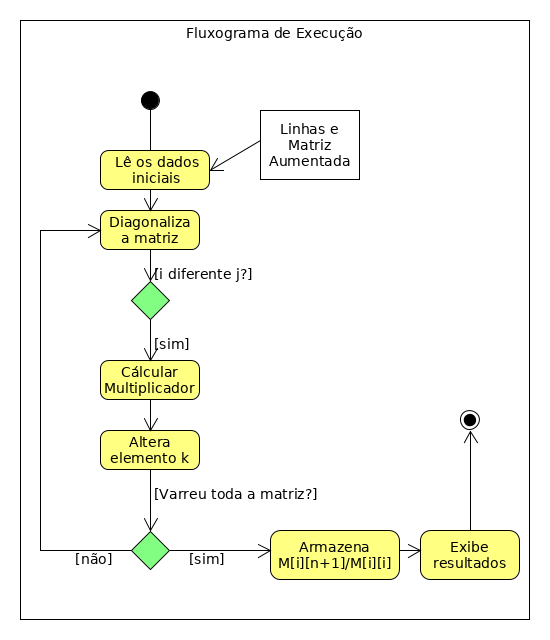
\includegraphics[width=10cm]{figuras/fluxograma.png}\\
  \caption{Fluxo de execução da solução}\label{fig:fluxo}
\end{figure}

A solução elaborada neste relatório funciona da seguinte maneira. É necessário inserir a quantiade de linhas
do sistema de equações lineares, em formato de matriz aumentada, que se quer resolver. Após isso o programa
solicitará a inserção dos elementos de cada uma das linhas da matriz. Após completar a matriz de entrada o
sistema irá fazer a diagonalização de acordo com o método de eliminação de Gaus-Jordan. Onde caso os índices
i e j sejam diferentes, ou seja não fazem parte da diagonal principal, será aplicado o algoritmo de eliminação.
Após haver apenas os elementos da diagonal principal, o método de solução se torna direto e com isso é possível
encontrar os valores da incógnitas que se busca. As limitações do programa são entradas de matrizes de no máximo
10x10 e apenas para equações lineares.

\newpage
\section{Código Fonte}

\lstinputlisting[language=C]{../solution/m2.c}

\newpage
\section{Resultados e discussões}

Nesta seção discutiremos os resultados obtido após a execução do programa.
O resultado encontrado a partir da solução proposta é condizente. Pois ao fazermos a comparação
do resultado obtido com o resultado de um site de solução de sistemas lineares (https://matrixcalc.org/pt/slu.html) ambos encontram
os mesmo valor, como pode ser visto abaixo:

\begin{figure}[!h]
  \centering
  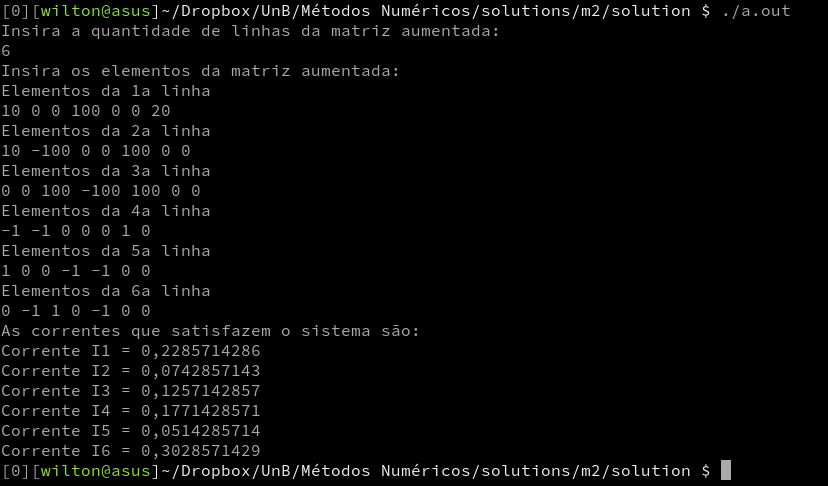
\includegraphics[width=15cm]{figuras/printx.png}\\
  \caption{Resultado da execução do programa}\label{fig:printx}
\end{figure}

\newpage
\begin{figure}[!h]
  \centering
  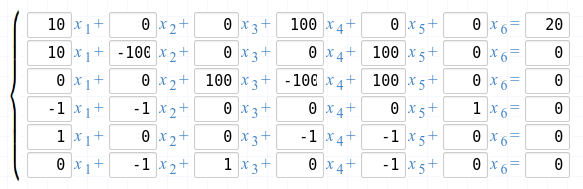
\includegraphics[width=15cm]{figuras/r1.png}\\
\end{figure}
\begin{figure}[!h]
  \centering
  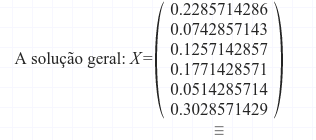
\includegraphics[width=10cm]{figuras/r2.png}\\
\end{figure}

Sendo assim, o objetivo proposto no início do relatório foi satisfatoriamente alcançado.

\newpage
\section{Ferramentas}
Todas as ferramentas utilizadas neste relatório são ferramentas open source (software livre).
Permitindo assim que qualquer um possa reproduzir e contestar as afirmações presentes neste documento.

\begin{enumerate}
  \item Arch Linux (\url{https://www.archlinux.org})
    \begin{itemize}
      \item Sistema operacional utilizado.
    \end{itemize}
  \item GCC (\url{https://gcc.gnu.org})
    \begin{itemize}
      \item Compilador de C utilizado para compilar a solução.
    \end{itemize}
  \item Python (\url{https://www.python.org})
    \begin{itemize}
      \item Linguagem de programação utilizada para conferir os valores da solução.
    \end{itemize}
  \item vim (\url{http://www.vim.org})
    \begin{itemize}
      \item Editor de texto.
    \end{itemize}
  \item \LaTeX~(\url{https://www.latex-project.org})
    \begin{itemize}
      \item Sistema tipográfico de alta qualidade (utilizado para elaborar o relatório).
    \end{itemize}
  \item Gnuplot (\url{http://www.gnuplot.info})
    \begin{itemize}
      \item Utilitário de representação gráfica (utilizado para plotagem do gráfico).
    \end{itemize}
  \item UMLet (\url{http://www.umlet.com})
    \begin{itemize}
      \item Ferramenta de UML (utilizado para criar o fluxo de execução).
    \end{itemize}
  \item Shutter (\url{http://shutter-project.org})
    \begin{itemize}
      \item Programa de captura de tela (utilizado para capturar os resultados).
    \end{itemize}
\end{enumerate}

%%%%%%%%%%%%%%%%%%%%%%%%%%%%%%%%%%%%%%%%%%%%%%%%%%%%%%%%%%%%%%%%%%%%%%%%%%%%%%%%%%%%%%%%%

\end{document}
